% 日本語の簡潔版（英語草稿 main.tex の要約）．Build: uplatex main_ja && uplatex main_ja && dvipdfmx main_ja
\documentclass[uplatex,dvipdfmx,a4paper,10pt,twocolumn]{jsarticle}
\usepackage[margin=18mm,columnsep=7mm]{geometry}
\usepackage{amsmath,amssymb,amsthm,bm}
\usepackage{booktabs}
\usepackage{graphicx}
\usepackage[dvipdfmx]{hyperref}
\graphicspath{{../figs/}}
\renewcommand{\topfraction}{0.9}\renewcommand{\dbltopfraction}{0.9}\renewcommand{\textfraction}{0.1}
\renewcommand{\floatpagefraction}{0.85}\renewcommand{\dblfloatpagefraction}{0.85}
\newtheorem{proposition}{命題}
\newtheorem{corollary}{系}

\title{量子リザバー PINN の公平な評価\\
\large ―固体力学と Phase-field 方程式―}
\author{西岡 佳祐\\{慶應義塾大学 理工学研究科}}
\date{草稿，\today}

\begin{document}
\makeatletter\twocolumn[\@maketitle\begin{center}\begin{minipage}{0.9\textwidth}\small\textbf{概要}\quad{}量子物理情報付きニューラルネットワーク（QPINN）は，パラメータが少なく精度もそこそこと報告されることが多いが，
同じ規模で同じだけ調整した古典モデルと比べた例は少ない．本研究は，線形弾性と Phase-field（PF）方程式を対象に，
対照をそろえてこの問いを調べる．
(1) 変分 QPINN は表現力ではなく最適化で詰まる．Allen--Cahn 方程式では 6 量子ビットの QPINN の誤差は 0.76 だった．
(2) 回路を固定し出力の係数だけを最小二乗で解く量子リザバー PINN（QERC-PINN）はこの問題を避け，Kirsch 問題で
$5\times10^{-5}$ に達する．
(3) リザバーは表現力を増やせないことを命題として示す．特徴量はエンコーディングで決まる関数空間 $\mathcal F_\rho$ の
部分空間を張るだけで，$\mathcal F_\rho$ は 1 量子ビットの関数の積で張られ，古典でも 1 特徴量あたり $O(N)$ の計算で作れる．
実機での読み出しには 1 点あたり $O(N^2 2^N/\varepsilon^2)$ ショットが要り，古典で計算するより高くつく．
(4) TSV（2 次元，軸対称，3 次元）と Allen--Cahn，Cahn--Hilliard で比べると，学習なしの最小二乗ソルバーは
公表されている適応 PINN より正確だが，量子リザバーは古典の乱数特徴量に負け，鋭い界面では量子ビットを増やしても
改善しない．\end{minipage}\end{center}\vspace{1em}]\makeatother

\section{はじめに}
PINN \cite{raissi} は PDE の残差をネットワークのパラメータについて最小化して解を求める．量子版の QPINN は，
少ないパラメータで大きな関数空間を表せることを利点とするが，その主張は比べる古典モデルに強く依存する．
本研究では「量子モデルのどの部分が役に立っているのか，同じ構造の古典モデルで再現できるのか」を問う．
対象は線形弾性（円孔板，半導体の貫通電極 TSV）と，界面が鋭く PINN が苦手とされる PF 方程式
（Allen--Cahn，Cahn--Hilliard）\cite{wight} である．

\paragraph{関連研究.} 古典では，固定の乱数特徴量で PDE の残差を最小二乗で解く PIELM \cite{pielm} や
乱数特徴量法 \cite{rfm}，それを時間発展に広げた方法 \cite{zhou} が高い精度を示している．
量子では，変分回路を学習する QPINN \cite{qcpinn,zabihi} と，量子リザバー \cite{ikeda} がある．
Zabihi ら \cite{zabihi} は古典 NN と量子回路の混成で Allen--Cahn の誤差が古典 PINN の約 5 分の 1 になると報告したが，
同じ規模の古典の対照とは比べていない．誤り耐性の量子計算機向けには，Carleman 線形化で反応拡散方程式を解く
アルゴリズム \cite{an,sasaki} がある．本研究は近い将来の機械向けの量子リザバーを，同じ解き方の古典の特徴量と比べる．

\section{手法}
\paragraph{最小二乗 PINN.} 解を固定の特徴量で $u(\bm x)=\sum_kc_k\varphi_k(\bm x)$ と展開し，PDE の残差・境界条件・
界面条件が係数 $\bm c$ について線形になることを使って，最小二乗を 1 回解く（PIELM \cite{pielm}）．
時間発展の PF 方程式では BDF2 で時間を進め，非線形項を Newton 法で線形化し，各反復で最小二乗を 1 回解く．
Cahn--Hilliard は化学ポテンシャル $\mu$ を未知数に加えた混合形で解く．

\paragraph{比べる特徴量.}
\begin{itemize}
  \item 量子リザバー：1 量子ビットごとのエンコーディング $|\psi(\bm x)\rangle=\bigotimes_l(\cos\frac{\theta_l}{2}|0\rangle+e^{i\theta_{N+l}}\sin\frac{\theta_l}{2}|1\rangle)$
        と固定の Haar ユニタリ $U$ から，$p_k=|\langle k|U|\psi\rangle|^2$（$2^N$ 個）
  \item 古典の乱数特徴量：$\tanh(\bm w_k\cdot\bm x+b_k)$，$\cos(\bm w_k\cdot\bm x+b_k)$
  \item 古典の対照：同じエンコーディングを使うテンソル積射影，積の乱数特徴量（命題 2）
  \item 学習あり：変分 QPINN と古典 PINN（Adam で学習）
\end{itemize}
どの特徴量も数は $2^N$ にそろえ，入力の倍率をシードごとに掃引して最良を採る．最良の倍率が探索範囲の端なら範囲を広げる．

\begin{figure*}[t]
\centering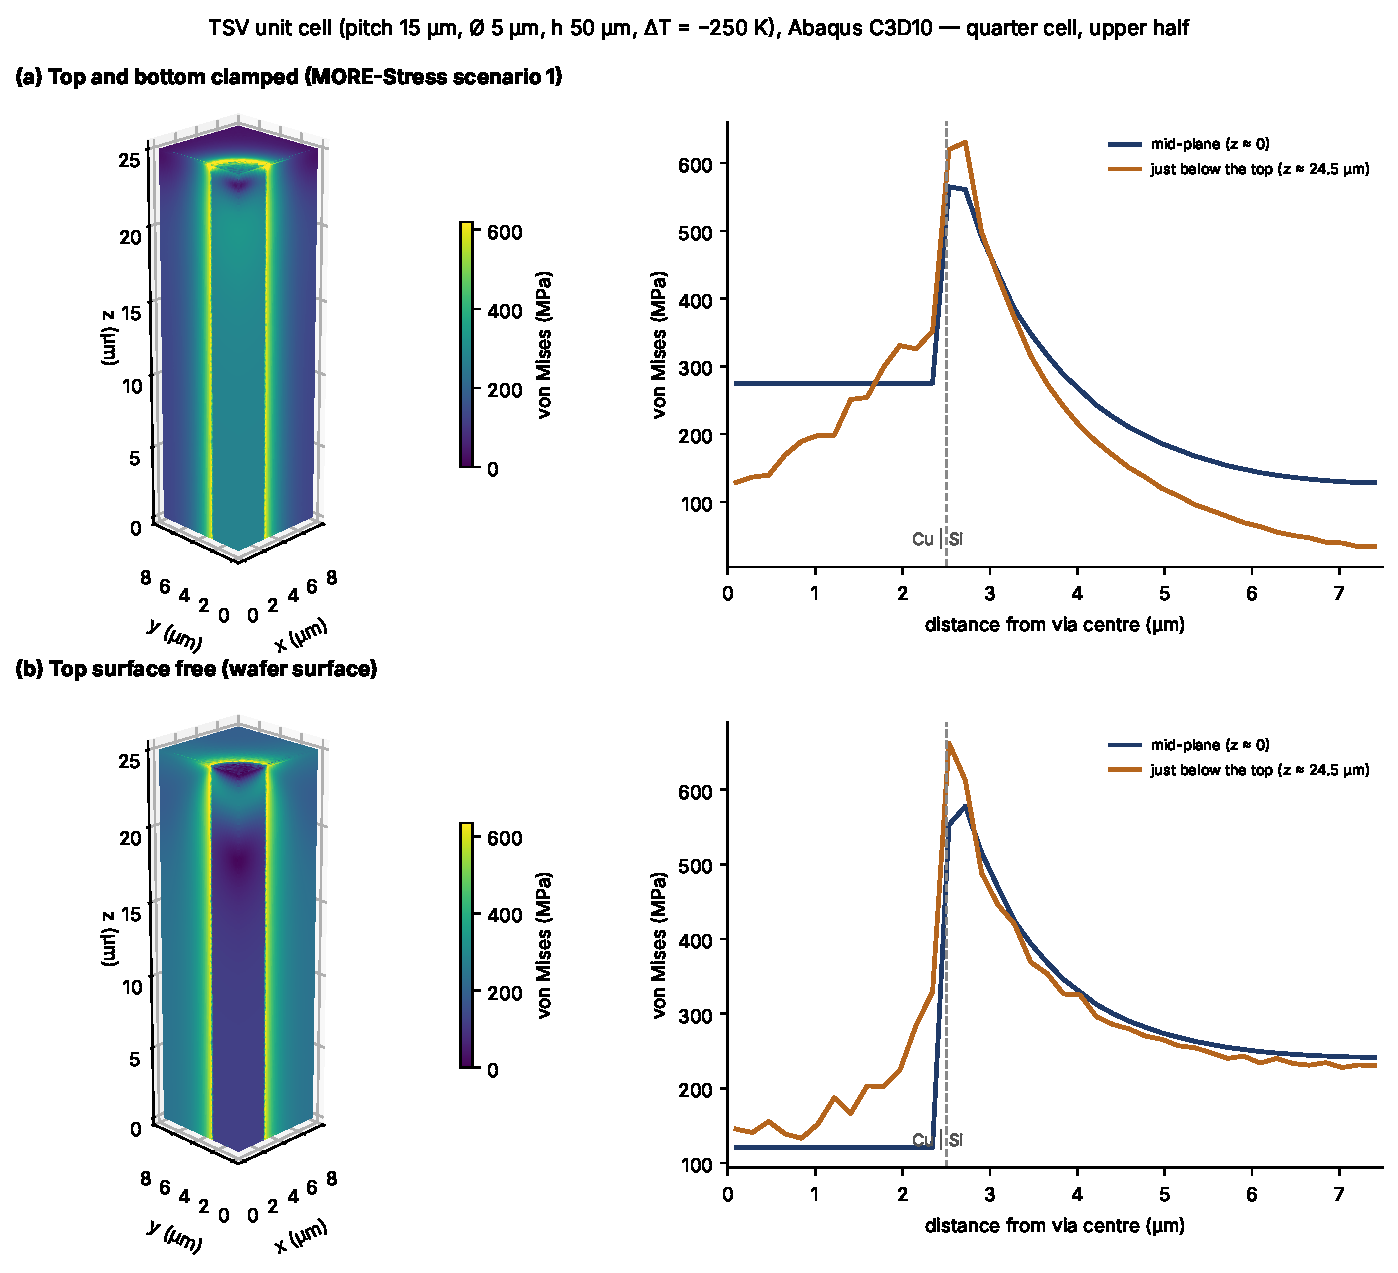
\includegraphics[width=0.75\textwidth]{tsv3d_abaqus.pdf}
\caption{TSV の単位セル（直径 5\,\textmu m，高さ 50\,\textmu m，ピッチ 15\,\textmu m，$\Delta T=-250$\,K）の Abaqus 参照解．
von Mises 応力は上面近くで大きく，2 次元の平面ひずみでは表せない．}
\end{figure*}

\section{理論：リザバーが加えられるもの}
$\rho(\bm x)=\bigotimes_l\rho_l(\bm x)$ とし，$\mathcal F_\rho=\{\mathrm{Tr}[H\rho(\bm x)]:H\ \text{エルミート}\}$ とおく．
\begin{proposition}
任意の $U$ に対し $\mathrm{span}\{p_k\}\subseteq\mathcal F_\rho$．リザバーは $\mathcal F_\rho$ の中から $2^N$ 次元の部分空間を選ぶだけである．
\end{proposition}
\begin{proposition}
$\mathcal F_\rho=\mathrm{span}\{\prod_l\mathrm{Tr}[A_l\rho_l(\bm x)]\}$（$A_l$ は $2\times2$ エルミート）．よって $\dim\mathcal F_\rho\le4^N$．
\end{proposition}
\begin{corollary}
積の乱数特徴量 $f_k=\prod_l\mathrm{Tr}[A_{k,l}\rho_l]$ は $\mathcal F_\rho$ に入り，古典で 1 個あたり $O(N)$ で計算できる．
\end{corollary}
\begin{proposition}
各 $p_k$ を $S$ ショットで推定すると相対誤差は約 $\sqrt{2^N/S}$．2 階微分にはパラメータシフトで $O(N^2)$ 個の回路が要り，
1 点あたり $O(N^2 2^N/\varepsilon^2)$ ショットになる．古典の積の特徴量は $O(N2^N)$ 回の演算で済む．
\end{proposition}
TSV 単体（$N=8$，3 シード）では，積の乱数特徴量が $3.5\times10^{-3}$，Haar リザバーが $3.9\times10^{-3}$ で，
古典の $O(N)$ の特徴量が同等以上だった．

\section{結果}
\subsection{固体力学}
\begin{figure*}[t]
\centering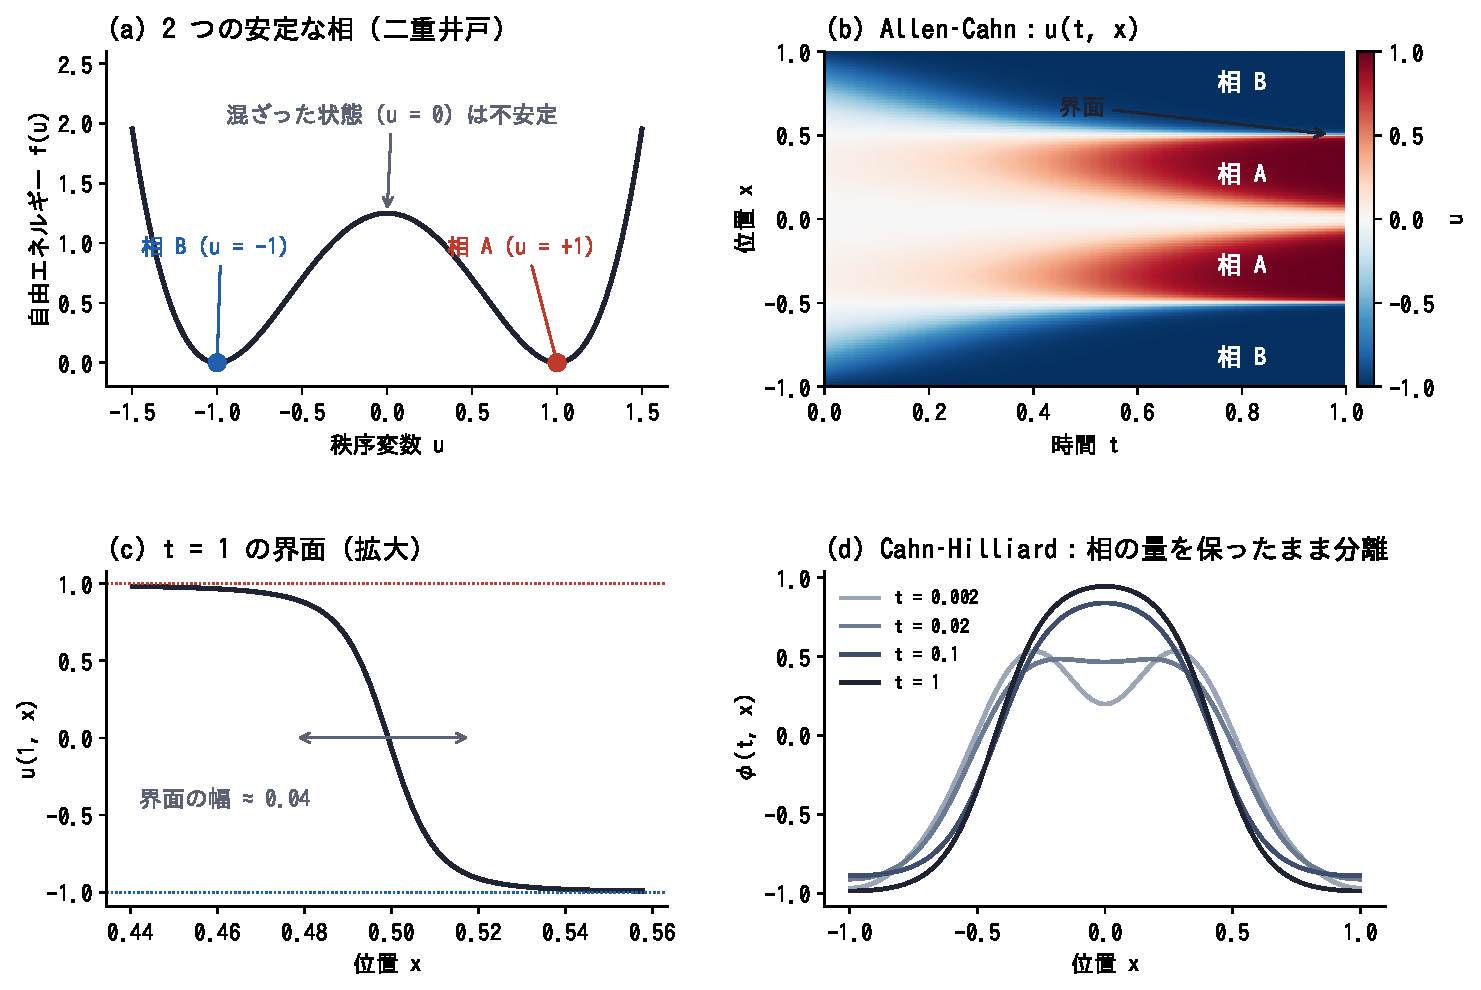
\includegraphics[width=0.72\textwidth]{pf_explain.pdf}
\caption{Phase-field 法の基本（計算した参照解から作図）．(a) 二重井戸の自由エネルギー，(b) Allen--Cahn の $u(t,x)$，
(c) $t=1$ の界面（幅 約 0.04），(d) Cahn--Hilliard は相の量（平均）を保ったまま分離する．}
\end{figure*}

\begin{table*}[t]
\centering\small
\caption{変位の相対 $L_2$ 誤差（シードごとに倍率を調整した幾何平均）}
\begin{tabular}{lcccc}
\toprule
問題 & 量子リザバー & テンソル積射影 & tanh & Fourier \\
\midrule
Kirsch 円孔板（$N=10$） & $4.6\times10^{-5}$ & -- & $5.9\times10^{-5}$ & $\bm{1.1\times10^{-6}}$ \\
TSV 単体（$N=8$）     & $4.6\times10^{-3}$ & $4.4\times10^{-3}$ & $4.8\times10^{-2}$ & $4.3\times10^{-2}$ \\
TSV 単体（$N=12$）    & $5.6\times10^{-5}$ & -- & $5.7\times10^{-5}$ & $\bm{8.3\times10^{-6}}$ \\
\bottomrule
\end{tabular}
\end{table*}
参照解は解析解，自作の有限要素法，Abaqus（CAX8, C3D10）で相互に $10^{-3}$ 以下で一致することを確認した．

\begin{table}[t]
\centering\small\setlength{\tabcolsep}{3pt}
\caption{参照解の相互確認（$\bm u$ は相対 $L_2$，von Mises は最大値で規格化した平均絶対誤差）}
\begin{tabular}{lccc}
\toprule
比較 & $\bm u$ & 中央面 & 上面近く\\
\midrule
軸対称・固定：自作 FE と Abaqus & 2.2e-4 & 3.2e-4 & 6.5e-4\\
軸対称・上面自由：同上 & 8.8e-5 & 3.2e-4 & 7.7e-4\\
3D 中央面 と 2D 平面ひずみ & 2.4e-4 & 3.1e-4 & --\\
\bottomrule
\end{tabular}
\end{table}
ビア中心の応力も平面ひずみの Lamé 解と一致した（$\sigma_{rr}=\sigma_{\theta\theta}=642$\,MPa，$\sigma_{zz}=917$\,MPa）．
入力の倍率の調整は結論を大きく変える．調整しない古典の対照は 2 シードでは量子と同等に見えたが，調整すると 20 倍良くなった．
また $N=12$ の Fourier 特徴量は，倍率の範囲を広げると $3.2\times10^{-4}$ から $8.3\times10^{-6}$ に改善した．
\begin{figure}[t]
\centering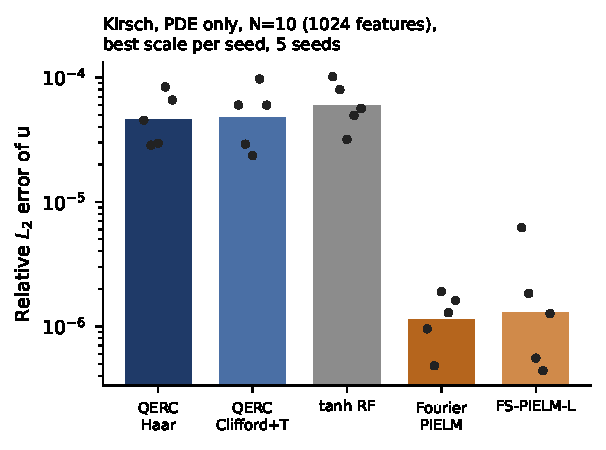
\includegraphics[width=\columnwidth]{qerc_fair_scales.pdf}
\caption{Kirsch 円孔板：すべての特徴量で入力の倍率を調整した比較（5 シード）．}
\end{figure}
量子リザバーは同じテンソル積構造の古典の対照と同等で，特徴量が増えると Fourier 特徴量が最良になる．
TSV の軸対称・3 次元セルでも Fourier 特徴量が最も正確だった．


\begin{table}[t]
\centering\small
\caption{TSV 軸対称セル（$N=8$，5 シード）：$\bm u$ の誤差と上面近くの von Mises の誤差}
\begin{tabular}{lcccc}
\toprule
 & \multicolumn{2}{c}{上下固定} & \multicolumn{2}{c}{上面自由}\\
特徴量 & $\bm u$ & 上面 & $\bm u$ & 上面\\
\midrule
量子 & 2.7e-2 & 9.8e-3 & 9.9e-3 & 2.0e-2\\
2 層 NN & 2.7e-2 & 8.8e-3 & 8.1e-3 & 2.1e-2\\
tanh & 1.5e-2 & 8.0e-3 & 3.2e-3 & 1.5e-2\\
Fourier & \textbf{6.0e-3} & \textbf{4.7e-3} & \textbf{1.5e-3} & \textbf{6.5e-3}\\
\bottomrule
\end{tabular}
\end{table}
上面近く（デバイスを置く領域）の誤差は中央面の 3〜15 倍で，どのモデルでも難しい．量子リザバーは乱数の 2 層ネットワークと同程度である．

\subsection{Phase-field 方程式}
\begin{figure}[t]
\centering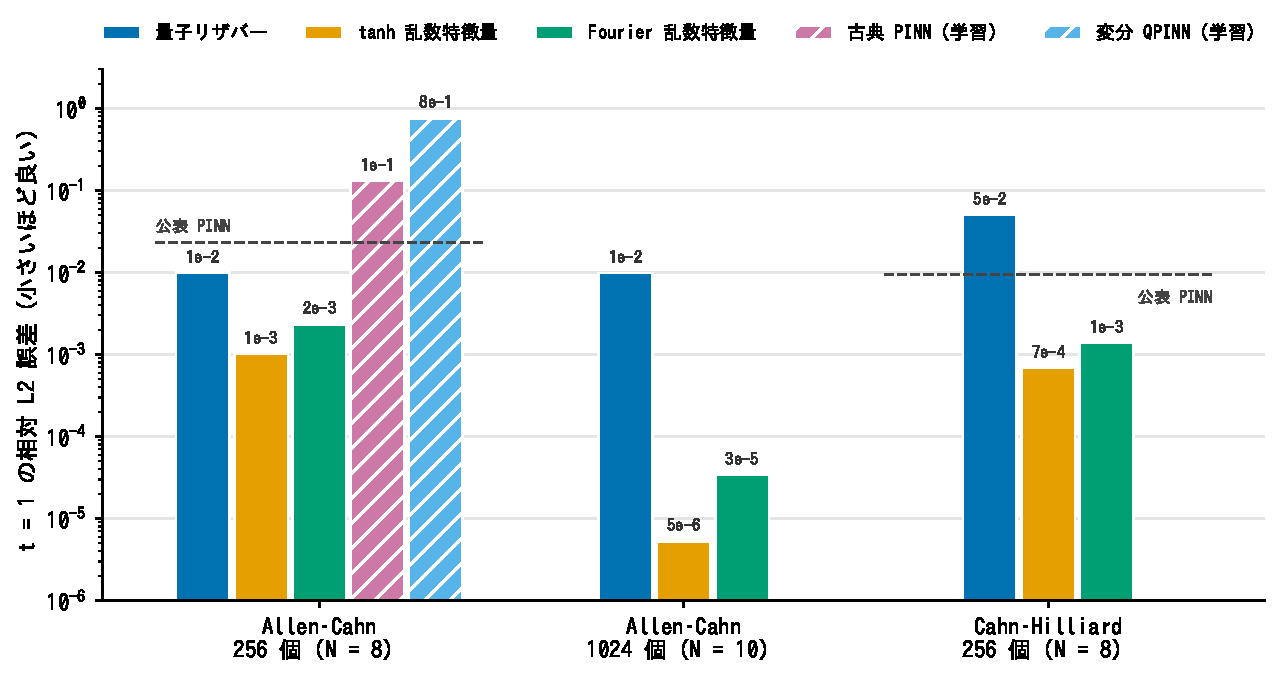
\includegraphics[width=\columnwidth]{pf_compare.pdf}
\caption{Phase-field 方程式での各手法の誤差（対数軸，低いほど良い）．破線は公表されている適応 PINN．}
\end{figure}

Allen--Cahn は Raissi らの例題 $u_t-10^{-4}u_{xx}+5u^3-5u=0$，$u(0,x)=x^2\cos\pi x$（周期境界），
Cahn--Hilliard は Wight \& Zhao の例題 $u_t=\mu_{xx}$，$\mu=0.01(u^3-u)-10^{-6}u_{xx}$，$u(0,x)=-\cos2\pi x$ を用いた．
参照解は Fourier スペクトル法と ETDRK4 で求めた．

\begin{table}[t]
\centering\small\setlength{\tabcolsep}{3pt}
\caption{$t=1$ での相対 $L_2$ 誤差}
\begin{tabular}{lccc}
\toprule
手法 & AC（$N=8$） & AC（$N=10$） & CH（$N=8$） \\
\midrule
量子リザバー（最小二乗）& $1.0\times10^{-2}$ & $9.9\times10^{-3}$ & $5.0\times10^{-2}$ \\
tanh（最小二乗）& $1.0\times10^{-3}$ & $\bm{5.3\times10^{-6}}$ & $\bm{6.9\times10^{-4}}$ \\
Fourier（最小二乗）& $2.3\times10^{-3}$ & $3.4\times10^{-5}$ & $1.4\times10^{-3}$ \\
変分 QPINN（学習）            & 0.76 & -- & -- \\
古典 PINN（学習）& 0.13 & -- & -- \\
適応 PINN \cite{wight} & $2.3\times10^{-2}$ & -- & $9.5\times10^{-3}$ \\
\bottomrule
\end{tabular}
\end{table}


学習なしの最小二乗ソルバーは，学習ありの PINN・QPINN より桁違いに正確で，公表されている適応 PINN よりも良い．
一方で量子リザバーは特徴量を 256 から 1024 個に増やしても $10^{-2}$ で止まり，古典の乱数特徴量（$5\times10^{-6}$）との差は
広がった．命題 2 のとおり $\mathcal F_\rho$ は角度の 1 次の三角関数の積でできており，空間の細かさは $N$ ではなく
入力の倍率で決まるため，鋭い界面を表しにくい．
どの手法でも自由エネルギーは毎ステップ単調に減少し，Cahn--Hilliard の質量も $10^{-4}$ 以下のずれで保存された．
また特徴量の行列は係数や初期条件によらないので，1 組の量子特徴量で 9 通りの Allen--Cahn 問題を解けた
（実機なら回路の測定は 1 回で済む）．

\begin{table}[t]
\centering\small
\caption{1 組の量子特徴量（$N=8$）で解いた 9 通りの Allen--Cahn（$t=1$ の誤差）}
\begin{tabular}{lccc}
\toprule
初期条件 & $D=10^{-4}$ & $3\times10^{-4}$ & $10^{-3}$\\
\midrule
$x^2\cos\pi x$ & 1.4e-2 & 6.5e-3 & 9.2e-4\\
$0.5\cos2\pi x$ & 9.6e-2 & 6.4e-2 & 2.8e-2\\
$0.3\sin\pi x+0.2\cos3\pi x$ & 4.3e-2 & 2.3e-2 & 5.0e-3\\
\bottomrule
\end{tabular}
\end{table}
界面が鋭い（$D$ が小さい，界面が多い）ほど誤差が大きい．

\subsection{ショットノイズ}
実機では $p_k$ とその微分をショット測定で推定する．$p_k\approx2^{-N}$ なので相対ノイズは $\sqrt{2^N/S}$ で，
2 階微分がそれを増幅する．1 階微分だけで済むエネルギー（Ritz）形にすると，どのショット数でも誤差が 3〜4 倍小さくなる
（表\ref{tab:shot}）が，$10^7$ ショットでも 1.4\% で，ノイズなしの値の 70 倍である．
\begin{table}[t]
\centering\small
\caption{Kirsch 円孔板（$N=10$）：1 回路あたりのショット数と誤差}\label{tab:shot}
\begin{tabular}{lcc}
\toprule
ショット数 & 強形式 & エネルギー形\\
\midrule
$10^3$ & 0.46 & \textbf{0.32}\\
$10^5$ & 0.25 & \textbf{0.083}\\
$10^7$ & 0.062 & \textbf{0.014}\\
$\infty$ & $6.3\times10^{-4}$ & $\bm{2.1\times10^{-4}}$\\
\bottomrule
\end{tabular}
\end{table}

\section{考察とまとめ}
\begin{itemize}
  \item 精度の大部分は量子からではなく，非凸の最適化を線形の最小二乗に置き換えたことから来る．
  \item 量子リザバーの表現力はエンコーディングで決まり，同じ空間は古典で安く作れる．実機の読み出しはさらに高くつく．
  \item 古典の比較対象の調整（入力の倍率）で結論が 1 桁以上変わるので，掃引範囲と最良値が範囲の内側であることを報告すべきである．
  \item 課題：ショットノイズ（エネルギー形で 3〜4 倍改善したが不十分），2 次元の PF 問題，問題に合わせて設計したリザバー．
\end{itemize}
量子リザバー PINN は動く PDE ソルバーであり，変分 QPINN の最適化の失敗を避け，PF 方程式では学習ありの PINN より正確である．
しかし公平に比べると，同じ解き方の古典の乱数特徴量と同等かそれ以下であり，量子の優位は示せない．

\begin{thebibliography}{11}
\bibitem{raissi} M. Raissi, P. Perdikaris, G. E. Karniadakis, J. Comput. Phys. 378 (2019) 686--707.
\bibitem{wight} C. L. Wight, J. Zhao, Commun. Comput. Phys. 29 (2021) 930--954.
\bibitem{pielm} V. Dwivedi, B. Srinivasan, Neurocomputing 391 (2020) 96--118.
\bibitem{rfm} J. Chen, X. Chi, W. E, Z. Yang, arXiv:2207.13380 (2022).
\bibitem{zhou} H. Zhou, Z. Fu, Y. Wang, X. Feng, arXiv:2604.25502 (2026).
\bibitem{qcpinn} A. Farea, S. Khan, M. S. Celebi, arXiv:2503.16678 (2025).
\bibitem{zabihi} K. Zabihi, H. Montazeri, A. S. J. Suiker, arXiv:2606.04679 (2026).
\bibitem{ikeda} A. Ikeda, A. Sakurai, K. Nemoto, M. Muramatsu, arXiv:2601.02150 (2026).
\bibitem{an} D. An, D. Fang, S. Jordan, J.-P. Liu, G. H. Low, J. Wang, Commun. Math. Phys. (2023).
\bibitem{sasaki} S. Sasaki, K. Endo, M. Muramatsu, Sci. Rep. 16 (2026) 11743.
\end{thebibliography}
\end{document}
